\documentclass[12pt,fleqn]{article}\usepackage{../../common}
\begin{document}

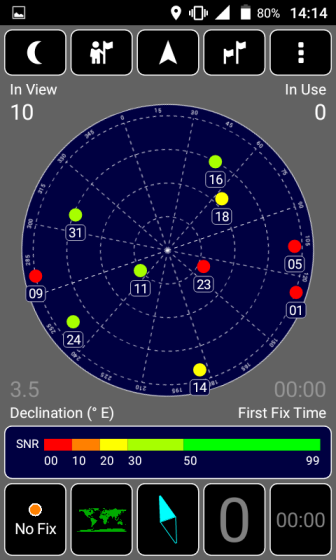
\includegraphics[width=20em]{gpstest.png}

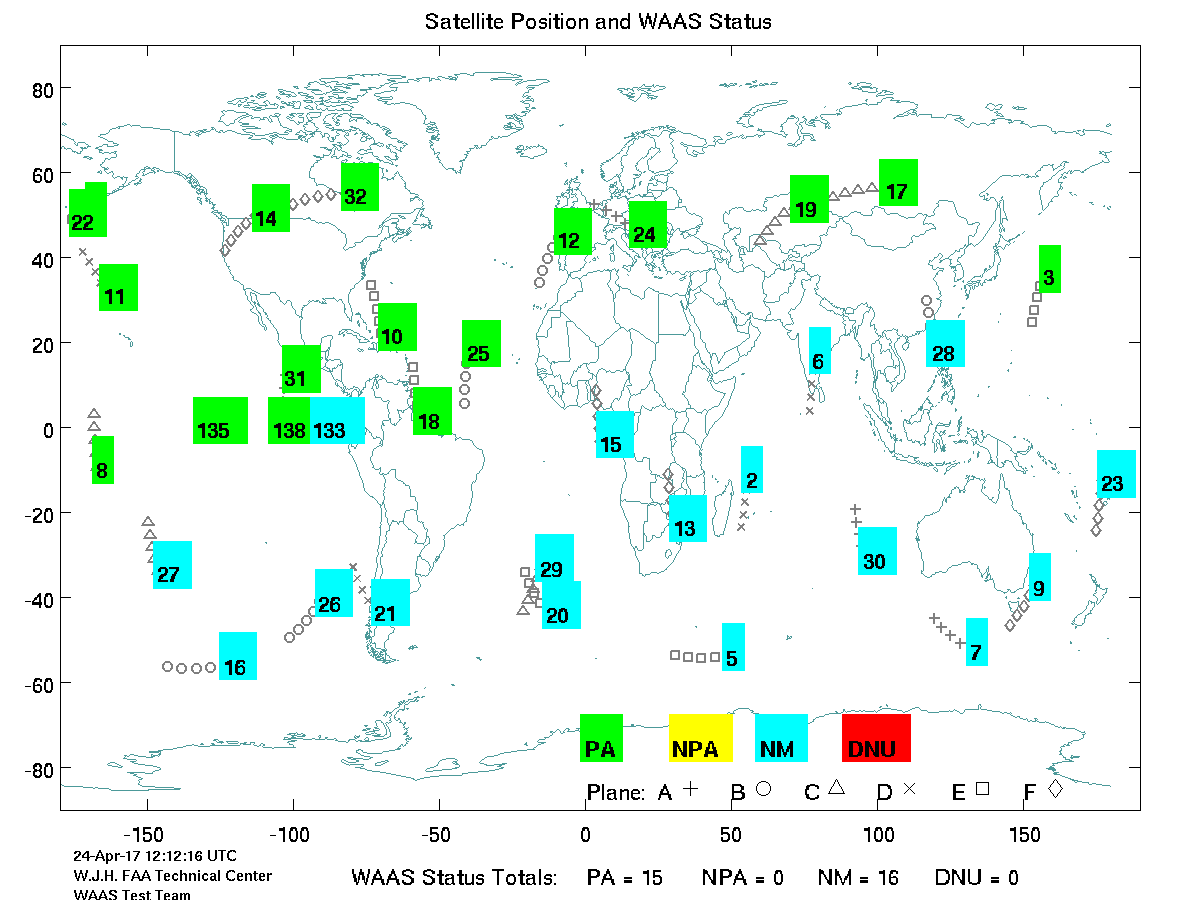
\includegraphics[width=40em]{waas_sats.png}

\inputminted[fontsize=\footnotesize]{python}{orbital.py}

\begin{minted}[fontsize=\footnotesize]{python}
import jdcal
print sum(jdcal.gcal2jd(dt.year, dt.month, dt.day))
\end{minted}

\begin{verbatim}
2457866.5
\end{verbatim}

\begin{minted}[fontsize=\footnotesize]{python}
from datetime import datetime
millis = 1493036068479
dt = datetime.fromtimestamp(millis/1000.0)
dtj = jdays(datetime.fromtimestamp(millis/1000.0))
print dtj
\end{minted}

\begin{verbatim}
2457868.09339
\end{verbatim}

\begin{minted}[fontsize=\footnotesize]{python}
sat_lon = -164.259351
sat_lat = 30.518234
sat_alt = 20*1000*1000
lon = 13.442383333333332
lat = 52.483086666666665
alt = 0
az,el = get_observer_look(sat_lon, sat_lat, sat_alt, dt, lon, lat, alt)
print az, el    
\end{minted}

\begin{verbatim}
358.005492414 -6.99245765159
\end{verbatim}









Kaynaklar 

[1] \url{http://www.nstb.tc.faa.gov/incoming/Waas_Sv_Status.txt}

\end{document}


